\documentclass[a4paper,12pt]{article} 
\usepackage[T2A]{fontenc}			
\usepackage[utf8]{inputenc}			
\usepackage[english,russian]{babel}	
\usepackage{amsmath,amsfonts,amssymb,amsthm,mathtools} 
\usepackage[colorlinks, linkcolor = blue]{hyperref}
\usepackage{upgreek}
\usepackage[left=2cm,right=2cm,top=2cm,bottom=3cm,bindingoffset=0cm]{geometry}
\usepackage{multirow}
\usepackage{graphicx}
\usepackage{xcolor}
\usepackage{multirow}

\author{Шелихов Дмитрий\\Группа Б01-305}

\title{\textbf{Работа 3.1.3\\Измерение магнитного поля Земли}} 
\date{\today}

\begin{document} 

\maketitle

\textbf{Цель работы:} исследовать свойства постоянных неодимовых магнитов; измерить с их помощью горизонтальную и вертикальную составляющие индукции магнитного поля Земли и магнитное наклонение.

\textbf{В работе используются:} неодимовые магниты; тонкая нить для изготовления крутильного маятника; медная проволока; электронные весы; секундомер; измеритель магнитной индукции; штангенциркуль; брусок; линейка и штатив из немагнитных материалов; набор гирь и разновесов.

\noindent\textbf{Теоретическая справка}

$$ \vec{m} = I\vec{S} $$ (1) - магнитный момент тонкого витка с током. 
$$ \vec {B_{дип}} = \frac {\mu_0}{4\pi}(\frac {3(\vec {m} \cdot \vec{r})\vec{r}}{r^5} - \frac {\vec{m}}{r^3})  $$ (2) - Магнитное поле точечного диполя. 
$$ \vec{M} = [\vec{m} \times \vec{B}]  $$ (3) - Механический момент сил, действующий на точечный магнитный диполь $\vec{m}$ 
$$ W = -(\vec{m} \cdot \vec{B})  $$ (4) - Потенциальная энергия, которой обладает диполь с постоянным $\vec{m}$
$$ \vec{F} = (\vec{m} \cdot \nabla)\vec{B}  $$ (5) - Сила, действующая на магнитный диполь в неоднородном внешнем поле $\vec{B}$.
$$ F_{12} = -\frac {6m_1m_2}{r^4}  $$ (6.1) - Сила, взаимодействия двух точечных диполей, когда их моменты направлены вдоль соединяющей их прямой.
$$ F_{12} = \frac {3m_1m_2}{r^4}  $$ (6.2) - Сила, взаимодействия, если моменты направлены перпендикулярно соединяющей их прямой.

\noindent\textbf{Экспериментальная установка}

Используем неодимовые шарообразные магниты: 
	а) Вещество магнитожёстко
	б) Шары намагничены однородно

$$ \vec {B_0} = \frac {\mu_0 \vec{m}}{2\pi R^3} $$ (7) - магнитное поле внутри шара (однородно).
$$ \vec {m} = \vec{M}V $$ (8), где $\vec{M}$ - намагниченность материала магнита.
$$ \vec {B_r} = 4\pi\vec{M}  $$ (9) - остаточная индукция материала. 
$$ B_p = B_0 = \frac {2}{3}B_r  $$ (10) - индукция на полюсах однородно намагниченного шара. 

\noindent\textbf{Определение магнитного момента магнитных шариков}

\textbf{Метод А.} 

Когда векторы двух магнитных моментов ориентированы вертикально: $$ \vec{m} = \sqrt{\frac{mg{r_{max}^4}}{6}} $$ (11) 

\center{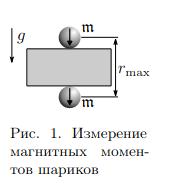
\includegraphics{1.png}}

\textbf{Метод Б.}

Максимальная сила сцепления определется по весу магнитной цепочки, которую способен удержать самый верхний магнитный шарик.

\center{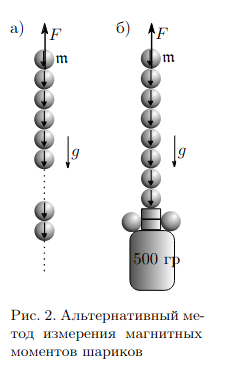
\includegraphics{2.png}}

Сила сцепления двух одинаковых шаров радиусами R с магнитными моментами $\vec{m}$ равна $$ F_0 = \frac{6m^2}{{(2R)}^4} = \frac{3m^2}{8R^4} $$ (12)

Минимальный вес цепочки, при котором она оторвётся от верхнего шарика, равен: $$ F = F_0(1 + \frac{1}{2^4} + \frac{1}{3^4} + \frac{1}{4^4} + ...) \approx 1,08F_0 $$ (13)

\textbf{Измерение горизонтальной составляющей индукции магнитного поля Земли}

Магнитное поле измеряем по периоду крутильных колебаний "магнитной стрелки" вокруг вертикальной оси. Стрелка стремится повернуться по горизонатльной составляющей магнитного поля Земли $\vec{B_{||}}$ в направлении Юг-Север. 

\center{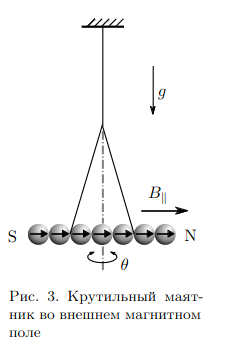
\includegraphics{3.png}}

$$ M = -m_nB_{||}sin\theta $$ (14)  - возвращающий момент сил. 

$$ J_n{\ddot{\theta}} + m_nB_{||}\theta = 0 $$ (15) - уравнение малых колебаний. 

$$ T = 2\pi \sqrt{\frac{J_n}{m_nB_{||}}}  $$ (16) - период малых колебаний. 

$$ J_n \approx \frac{1}{12}m_n{l_n}^2 = \frac{1}{3}n^3mR^2  $$ (17) - момент инерции магнитной стрелки. 

$$ T_n = 2\pi\sqrt{\frac{mR^2}{3mB_{||}}} \cdot n $$ (18) - период колебаний пропорционален числу шаров n, составляющих "стрелку". 

\textbf{Измерение вертикальной составляющей индукции магнитного поля Земли. Магнитное наклонение}

Подвешиваем стрелку в одной точке. $\beta$ - магнитное наклонение

С помощью доп. груза выравниваем стрелку по горизонтали.  

$$ M_n = m_{гр}gr_{гр} = nmB_{\perp}  $$ (19) - момент силы тяжести, уравновешивающего груза. 
Из равенства (19) определяем вертикальную составляющую индукции магнитного поля Земли. 

\center{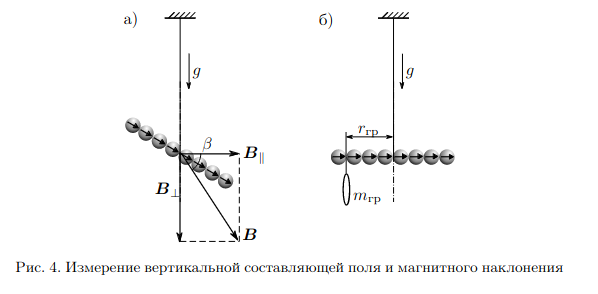
\includegraphics{4.png}}  

\textbf{Ход работы}

I. Определение магнитного момента, намагниченности и остаточной магнитной индукции вещества магнитных шариков. 

1) Измерим диаметр шариков и их массу.

\begin{center}
\begin{tabular}{|c|c|c|}
	\hline
	M, г (76 шаров) & m, г & $\Delta m$, г \\
	\hline
	63,316 & 0,833 & 0,001 \\
	\hline
\end{tabular}
\end{center}
\qquad
\begin{center}
\begin{tabular}{|c|c|}
	\hline
	& d, мм \\
	\hline
	& 5,496 \\
	\hline
	& 5,487 \\
	\hline
	& 5,492 \\
	\hline
	<d>, мм & 5,492 \\
	\hline
	$\Delta$ d, мм & 0,004 \\
	\hline
	d, мм & 5,492 $\pm$ 0,004 \\
	\hline
\end{tabular}
\end{center}

2) С помощью магнитометра измерим индукцию поля $B_p$ на полюсах шарика 

\begin{center}
\begin{tabular}{|c|c|}
	\hline
	N & $B_p$, мТл \\
	\hline
	1 & 357 \\
	\hline
	2 & 319 \\
	\hline
	3 & 275 \\
	\hline
	4 & 305 \\
	\hline
	5 & 346 \\
	\hline
	6 & 265 \\
	\hline
	7 & 368 \\
	\hline
	8 & 367 \\
	\hline
	9 & 357 \\
	\hline
	10 & 354 \\
	\hline
	11 & 400 \\
	\hline
	12 & 393 \\
	\hline
	<$B_p$>, мТл & 342 \\
	\hline
	$\sigma_{B_p}$, мТл & 41 \\
	\hline
	$B_p$, мТл & 342 $\pm$ 41 \\
	\hline
\end{tabular}
\end{center}

3) Определим максимальное расстояние $r_{max}$, на котором шарики удерживают друг друга в поле тяжести Земли.

\begin{center}
\begin{tabular}{|c|c|}
	\hline
	N & $r_{max}$, мм \\
	\hline
	1 & 22,5 \\
	\hline
	2 & 21,0 \\
	\hline
	3 & 22,5 \\
	\hline
	4 & 21,5 \\
	\hline
	5 & 22,5 \\
	\hline
	6 & 21,5 \\
	\hline
	7 & 19,0 \\
	\hline
	8 & 22,0 \\
	\hline
	9 & 21,5 \\
	\hline
	10 & 23,0 \\
	\hline
	<$r_{max}$>, мм & 21,7 \\
	\hline
	$\sigma_{r_{max}}$, мм & 1,1\\
	\hline
	$r_{max}$, мм & 21,7 $\pm$ 1,2 \\
	\hline
\end{tabular}
\end{center}

4) Рассчитаем величину магнитного момента магнитика m по формуле (11). Оценим погрешность 

$$ \varepsilon_m = \frac{1}{2}(\varepsilon_m + 4\varepsilon_{r_{max}})  $$

\begin{center}
\begin{tabular}{|c|c|c|c|c|}
	\hline
	m, г & g, $\frac{см}{с^2}$ & $r_{max}, см$ & m, ед.СГС & $\Delta$m, ед.СГС \\
	\hline
	0,833 & 981,5 & 2,17 & 54,95 & 6,11 \\
	\hline
\end{tabular}
\end{center}

5-6) Используя дополнительные шарики, составим цепочку из 23 шариков и подсоединим цепочку к гире и разновесам так, чтобы общая масса системы составила ~ 500 г. Подберём минимальный вес системы цепочки с гирей, при котором она отрывается от верхнего шарика. Оценить максимальную нагрузку таким методом получилось с точностью до 20 грамм.  

\begin{center}
\begin{tabular}{|c|c|c|c|c|}
	\hline
	$M_{нагр}, г$ &  N, шт & $M_{цеп}, г$ & $M_{общ}, г$ & $\Delta$M \\
	\hline
	539 & 23 & 19,16 & 558 & 20 \\
	\hline
\end{tabular}
\end{center}

7) Рассчитаем силу сцепления двух шаров и по ней определим магнитный момент шарика $\vec{m}$. Оценим погрешность результата по формуле $$ \varepsilon_m = \frac{1}{2} \cdot (\varepsilon_{M_{общ}} + 4 \cdot \varepsilon_d) $$

\begin{center}
\begin{tabular}{|c|c|c|c|c|c|c|}
	\hline
	$M_{общ}, г$ & g, см/$c^2$ & d, см & m, ед.СГС & $\varepsilon_{M_{общ}}$ & $\varepsilon_d$ & $\Delta$m, ед.СГС \\
	\hline
	557,03 & 981,5 & 0,5492 & 87,61 & 0,036 & 7,3 $\cdot 10^{-4}$ & 3,13 \\
	\hline
\end{tabular}
\end{center}

8) Итого, мы получили два различных значения магнитных моментов: 
\begin{center}
\begin{tabular}{|c|c|}
	\hline
	Способ А & Способ Б \\
	\hline
	m = (54,95 $\pm$ 6,11) ед.СГС & m = (87,61 $\pm$ 3,13) ед.СГС \\
	\hline
\end{tabular}
\end{center}

Исходя из полученных данных второй метод обладает меньшей погрешностью. 
По табличным данным для данного материала остаточная индукция $B_r$ = 12200 Гаусс, что соответствует m = 85 ед.СГСЭ для шариков диаметром d = 5,5 мм. 
Исходя из этого, далее будем считать правильными данные, полученные в методе Б.

9) Рассчитаем величину намагниченности материала шариков M и остаточную индукцию магнитного поля $B_r$. Проведем сравнение с табличными значеними. 

\begin{center}
\begin{tabular}{|c|c|c|c|c|c|}
	\hline
	d, мм & V, мм3 & m, ед.СГС & M, ед.СГС & $B_r$, кГс & $B_{r_{табл}}$, кГс \\
	\hline
	5,492 $\pm$ 0,004 & 86,734 $\pm$ 0,190 & 87,61 $\pm$ 3,13 & 1010 $\pm$ 10 & 12,7 $\pm$ 0,1 & 12,2-12,5\\
	\hline
\end{tabular}
\end{center}

Видим, что полученные данные отличаются от табличных всего на 0.8 - 5\%. Это подтверждает, что метод Б более точный, чем метод А. Незначительное расхождение с табличным значением может быть вызвано отличием магнитного момента $\vec{m}$ самого верхнего шарика цепочки от среднего значения. Это различие может достигать 12\%! Опыт следовало проводить меняя верхний шарик местами с другими шариками цепи, усредняя магнитный момент шарика сверху.

10) Рассчитаем индукцию $B_p$ у полюсов шарика. Сравним рассчётное значение $B_p$ с измеренным.

\begin{center}
\begin{tabular}{|c|c|}
	\hline
	$B_{p_{измеренное}}$, мТл & $B_{p_{рассчётное}}$, мТл \\
	\hline
	342 $\pm$ 41 & 84,7 $\pm$ 0,7 \\ 
	\hline
\end{tabular}
\end{center}

\end{document}

